\section{Reglerentwurf}
\subsection{Stationärer Zustand und Fehler}
Die UTF des offenen Regelkreises setzt sich dabei aus derjenigen von Strecke
und Regler zusammen: $G_0(s) = G_S(s)G_R(s)$. Es wird davon ausgegangen, dass G0
vollständig gekürzt ist und vom Typ $\nu$ ist d.h. $\nu$ offene Integratoren hat, bzw. $\nu$ Pole
bei Null:
\begin{table}[h!]
	\begin{tabularx}{\textwidth}{|l||X|X|X|}
	\hline
		& $r(t)=\varepsilon(t) \quad $ Sprung & $r(t)=t \quad$ Rampe & $r(t)=\frac{t^2}{2} \quad$ Parabel \\ \hline\hline
		$\nu =0 \ (Typ \ 0) \quad P-Verhalten$ & $e_\infty=\frac{1}{1+K_0}$ & $e_\infty=\infty$ & $e_\infty=\infty$ \\ \hline
		$\nu =1 \ (Typ \ 1) \quad  I-Verhalten$ & $e_\infty=0$ & $e_\infty=\frac{1}{K_0}$ & $e_\infty=\infty$ \\ \hline
		$\nu =2 \ (Typ \ 2) \quad  I^2-Verhalten$ & $e_\infty=0$ & $e_\infty=0$ & $e_\infty=\frac{1}{K_0}$ \\ \hline
	\end{tabularx}
\end{table}
\subsection{Spezifikationen für das dynamische Verhalten}
\begin{eqnarray}
	G_f(s)=\frac{Y(s)}{R(s)}=\frac{G_0(s)}{1+G_0(s)} \\
	S(s)=\frac{1}{1+G_0(s)}\\
	T(s)=1-S(s)=\frac{G_0(s)}{1+G_0(s)}
\end{eqnarray}
\begin{figure}[h!]
	\begin{center}
	\begin{subfigure}[b]{8cm}
		\centering
		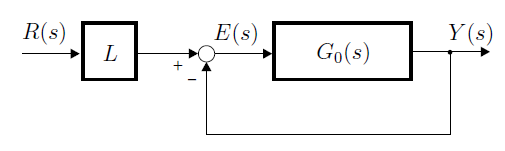
\includegraphics[width=8cm]{./images/regelkreismitL.png}
		\caption{Regelkreis mit Einheitsrückführung und Vorverstärkung L}
	\end{subfigure}\qquad
	\begin{subfigure}[b]{8cm}
		\centering
		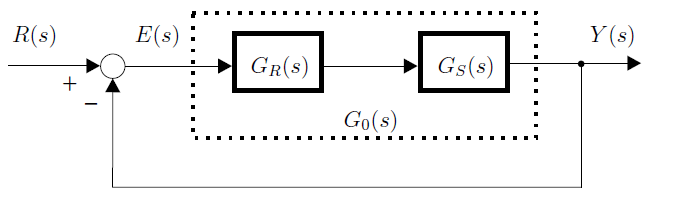
\includegraphics[width=8cm]{./images/RegelkreisEinheitsrueckfuehrung.png}
		\caption{Regelkreis mit Einheitsrückführung}
	\end{subfigure}
	\end{center}
\end{figure}\\
	Wird z.B. die Führungsgrösse mit einem Faktor bzw. Vorfilter L(s) vorverstärkt so ist $G_f(s)=\frac{Y(s)}{R(s)}=L(s)\cdot\frac{G_0(s)}{1+G_0(s)}$ während S(s) und T(s) erhalten bleiben.

\subsection{Restriktionen: Bode-Integral der Sensitivität}

beim Erhöhen der Bandbreite $\omega_B$
die Gefahr besteht, dass in den Amplitudengängen von T und S Überhöhungen
entstehen. Werden T und S gemäss Abb. 63 als UTF T(s) = Y(s)/R(s) und
S(s) = E(s)/R(s) = Y (s)/Z(s) interpretiert, so ist auch klar, dass diese Überhöhungen
nachteilig sind. Oft wird deshalb die Spezifikationen ergänzt durch Maximalwerte für die Resonanzüberhöhung von
T und/oder S. Typische Maximalwerte sind z.B. 3-5 dB.
\begin{equation}
\int\limits_{0}^{\infty}ln|S(j\omega)|d\omega =\underbrace{\pi\cdot\sum\limits_{i=1}^{N_{p}}Re(p_i)}
\label{BodeIntegral}
\end{equation}
\textcolor{white}{x} \hspace{9.5cm} 0, falls $G_0$ stabil 
\begin{itemize}
	\item Die Bedingung $n-m \geq 2$ ist in einem Regelkreis erfüllt, weil realistischerweise
	sowohl Strecke wie Regler Tiefpassverhalten zeigen.
	\item Ist $G_0$ stabil, dann wird der Ausdruck in (\ref{BodeIntegral}) gleich Null. Ist bei einer Frequenz
	$|S(j\omega)| < 0 \ dB$, dann muss zwingend irgendwo anders $|S(j\omega)| > 0 \ dB$ sein.
	\item Verkleinert man $|S(j\omega)|$ an einer Stelle, wird $|S(j\omega|$ dafür an einer anderen
	Stelle grösser; dies wird als ‘Wasserbetteffekt’ bezeichnet.
	Gleichung (\ref{BodeIntegral}) hat den Charakter eines Erhaltungsgesetzes.
	\item Ist $G_0$ instabil, dann verschlechtert sich die Situation entsprechend.
	\item Bei den Frequenzen, bei denen
	der Aushub für ein bessere Bandbreite $\omega_B$ abgelagert wird, muss der Abstand zwischen dem Punkt -1 und der
	Ortskurve, d.h. $|1 + G_0|$, im Intervall $1 > |1 + G_0| \geq (1 + \varepsilon)-1$ liegen.
\end{itemize}

In der Praxis kann der Aushub also nicht einfach in einem beliebig hohen bzw.
breiten Frequenzband ‘entsorgt’ werden, sondern man muss Gleichung (\ref{BodeIntegral}) etwas
einschränken:
\begin{equation}
\int\limits_{0}^{\omega_M}ln|S(j\omega)|d\omega =\pi\cdot\sum\limits_{i=1}^{N_{p}}Re(p_i)
\end{equation}